% This is part of Un soupçon de mathématique sans être agressif pour autant
% Copyright (c) 2012
%   Laurent Claessens
% See the file fdl-1.3.txt for copying conditions.

\begin{corrige}{Seconde-0037}


\begin{enumerate}

\item Le tableau suivant donne les effectifs cumulés croissants de cette série.  

  \begin{tabular}{|c||c|c|c|c|c|c|c|c|c|c|}
    \hline 
    \textbf{Salaire} &900&1\,100&1\,300&1\,500&1\,700&1\,900&2\,100&2\,500&3\,100&4\,500\\
    \hline 
    \textbf{Effectif} &12&10&20&18&8&8&5&5&2&1\\
    \hline 
    \textbf{ECC} &12&22&42&60&68&76&81&86&88&89\\
    \hline
  \end{tabular}
  
  \medskip
  Cette entreprise a $89$ salariés.
  \smallskip

\item Le calcul du salaire moyen brut noté $\bar{s}$ donne
  \begin{align*}
    \bar{s} &= 
    \frac{900\times 12 + 1\,100\times 10 + 1\,300\times 20 + \ldots+
      2\,500\times 5 + 3\,100\times 2 + 4\,500}{89}\\
    \bar{s} &\approx 1\,543
  \end{align*}
  Le salaire moyen brut de cette entreprise est de $1\,543$ euros environ.
  \smallskip

\item L'étendue du salaire dans cette entreprise est de
  $4\,500-900=3\,600$ euros.

\item L'effectif total (89) est impair, le salaire médian est donc la
  donnée de rang $45$ (valeur arrondie par excès de $89 / 2 = $ 44,5),
  ce qui donne un salaire médian de $1\,500$ euros.

  Le premier quartile est la donnée de rang $23$ (valeur arrondie par
  excès de $89 / 4 =$ 22,25), ce qui donne $Q_1 = 1\,300$ euros.

  Le troisième quartile est la donnée de rang $67$ (valeur arrondie
  par excès de $(3\times89) / 4 = $ 66,75), ce qui donne $Q_3 = 1\,700$
  euros.

\item Le nombre de salaires compris dans l'intervalle interquartile
  est le nombre de salaires compris entre 1\,300 euros (inclus) et
  1\,700 euros (inclus). Il y en a donc : $20+18+8=46$, soit un
  pourcentage du total correspondant à $\frac{46}{89}\times100\approx
  52$ \% en arrondissant à 1 \% près comme demandé.

\item Le diagramme en boîte de la série des salaires est le suivant :

    \begin{center}
    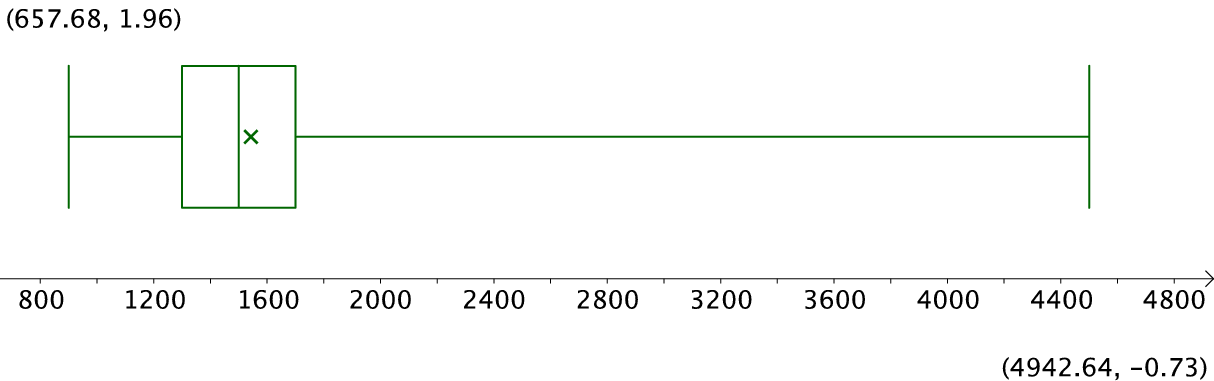
\includegraphics[width=10cm]{DS8_FigCor_Ex2}
    \end{center}
  
  La croix représente le salaire moyen.

\item Cette erreur ne concerne pas les valeurs extrêmes de la série et
  ne change donc pas l'étendue de la série qui reste de $3\,600$
  euros.

  Le salaire médian est toujours la donnée de rang $45$ de la série,
  qui reste toujours égale à $1\,500$ euros d'après le tableau
  ci-dessous où l'on a commencé à calculer les effectifs cumulés
  croissants : 


  \begin{center}
  \begin{tabular}{|c||c|c|c|c|c|c|c|c|c|c|}
    \hline 
    \textbf{Salaire} &900&1\,100&1\,300&1\,500&1\,700&1\,900&2\,100&2\,500&3\,100&4\,500\\
    \hline 
    \textbf{Effectif} &12&10&20&8&18&8&5&5&2&1\\
    \hline 
    \textbf{ECC} &12&22&42&50&&&&&&\\
    \hline
  \end{tabular}
  \end{center}

  Le salaire médian ne change donc pas.

  \smallskip

  En revanche, le salaire moyen augmente, puisque dix salaires sont
  passés de 1\,500 à 1\,700 euros.
  
\end{enumerate}


\end{corrige}
